\documentclass[t]{beamer}

% Load general definitions
% Preamble file - general definitions, package loading, etc.

%=================================
% Load packages
\usepackage{amssymb,amsmath}
\usepackage{graphicx}
\usepackage{url}
\usepackage{tikz}
\usetikzlibrary{mindmap,trees,arrows}
\usepackage{fancyvrb}
\usepackage[english]{babel}
\usepackage[latin1]{inputenc}
\usepackage{subfigure}
\usepackage{times}
\usepackage[T1]{fontenc}
\usepackage{cancel}
\usepackage{color}
\usepackage{listings}

%=================================
% Set mode
\mode<presentation>
{
	\usetheme{Madrid}
	\usecolortheme{whale}
	\useoutertheme{infolines}
	\setbeamercovered{invisible}
}

% Get rid of nav bar
\beamertemplatenavigationsymbolsempty

% Insert frame number at bottom of the page.
\usefoottemplate{\hfil\tiny{\color{black!90}\insertframenumber}} 

%=================================
% Define new commands

\newcommand\Real{{\mathbb{R}}}
%\newcommand{\vi}{\vspace{0.6\baselineskip}}
%\newcommand{\goodgap}{\hspace{\subfigtopskip}\hspace{\subfigbottomskip}}


% Equation environments
\newcommand{\beq}{\begin{equation}}
\newcommand{\eq}{\end{equation}}
\newcommand{\beqs}{\begin{equation*}}
\newcommand{\eqs}{\end{equation*}}
\newcommand{\beqn}{\begin{eqnarray}}
\newcommand{\eqn}{\end{eqnarray}}

% Bold variables
\newcommand{\mbf}[1]{\ensuremath{\mathbf{#1}}}

% Itemization
\newcommand{\bitem}{\begin{itemize}}
\newcommand{\eitem}{\end{itemize}}
\newcommand{\spitem}{\vskip 1em\item}
\newcommand{\bitems}{\begin{itemize}\item}
\newcommand{\benums}{\begin{enumerate}\item}
\newcommand{\eenum}{\end{enumerate}}

% color blocks
\newenvironment{colorblock}[2]{%
\setbeamercolor{block title}{#2}
\begin{block}{#1}}{\end{block}}

% Vertical spacing
\newcommand{\vone}{\vskip 1em}
\newcommand{\vhalf}{\vskip .5em}

% Frame environments
\newenvironment{ftst}[3][t]{%
\begin{frame}{environment=ftst,#1}
\frametitle{#2}
\framesubtitle{#3}}{\end{frame}}

\newenvironment{ftstf}[2]{
\begin{frame}[fragile,environment=ftstf]
\frametitle{#1}
\framesubtitle{#2}}{\end{frame}}

% colors
\definecolor{MyGray}{rgb}{0.5,0.5,0.5}
\definecolor{MyDBGray}{rgb}{0.1,0.1,0.4}
\definecolor{darkgreen}{rgb}{0,0.4,0}
\definecolor{black}{rgb}{0,0,0}
\def\defn#1{{\color{red} #1}}

% Footnote
\renewcommand{\thefootnote}{\alph{footnote}}

% Relaxed footnotes
\newcommand{\lfr}[1]{\let\thefootnote\relax\footnote{\tiny #1}}

% Verbatim environment - using FANCYVRB package
\DefineVerbatimEnvironment%
{rcode}{Verbatim}
{fontsize=\scriptsize}

% Verbatim environment - using LISTINGS package
%\lstnewenvironment{rcode} {\lstset{	language = R,
%									basicstyle = \scriptsize\ttfamily,
%									showspaces = false,
%									showstringspaces = false,
%									showtabs = false,
%									keywordstyle = \color{black}\bfseries,
%									commentstyle = \color{darkgreen},
%									numbers = none,
%									otherkeywords={	<-,
%													ggplot,
%													geom_boxplot,
%													facet_grid,
%													shapiro.test,
%													fligner.test,
%													glht,
%													with},
%									deletekeywords={data,
%													model,
%													residuals,
%													c,
%													axis,
%													default,
%													labels,
%													qq.text}}}%
%{}


% Specific definitions
\title[]{Design and Analysis of Experiments}
\subtitle[]{03 - Point Estimators}
\author[]{Felipe Campelo\\{\footnotesize http://www.cpdee.ufmg.br/\textasciitilde fcampelo}}
\institute{Graduate Program in Electrical Engineering}
\date{\scriptsize Belo Horizonte\\March 2018}

\begin{document}

% cover page
\setbeamertemplate{footline}{}
\begin{frame}
\begin{flushright}

\includegraphics[width=.25\textwidth]{../figs/principal_completa3_ufmg}
\end{flushright}
  \titlepage
  \begin{tikzpicture}[remember picture,overlay]
  \node[anchor=south east,xshift=-5pt,yshift=122pt] at (current page.south east) {\tiny Version 2.12.2018};
  \node[anchor=south west,yshift=0pt] at (current page.south west) {
\includegraphics[width=.15\textwidth]{../figs/by-nc-sa.png}};
  \end{tikzpicture}  
\end{frame}

%=====

% quotation page
  \begin{frame}[b]
		\frametitle{}
\begin{columns}[T]
\column{0.77\textwidth}
\flushright{\small ``\textit{I like to think of ideas as potential energy.\\
										They're really wonderful, but nothing will happen\\
										until we risk putting them into action.}''\\\vspace{1em}
Mae Carol Jemison (1956 - )\\
American engineer, physician and astronaut}
\column{0.23\textwidth}
\begin{tikzpicture}[remember picture,overlay]
\node[anchor=south east,yshift=20pt,xshift=0pt] at (current page.south east)
{
\includegraphics[width=\textwidth]{../figs/MaeJamison.jpg}};
\end{tikzpicture}
\end{columns}
\vhalf
\lfr{Image by Monique Dong: \url{https://www.rainbowresource.com/viewpict.php?pid=065272}}
\end{frame}

%=====

% Main slides
\begin{ftst}
{Introduction}
{Probability vs. Statistics}
\textbf{Statistical inference}: using \textit{samples} to draw conclusion about \textit{populations};

\begin{columns}[T]
\column{0.48\textwidth}
	\begin{block}{Probability}
		\centering Given the pool,what are the odds of drawing a certain combination of colors?\\
		\centering 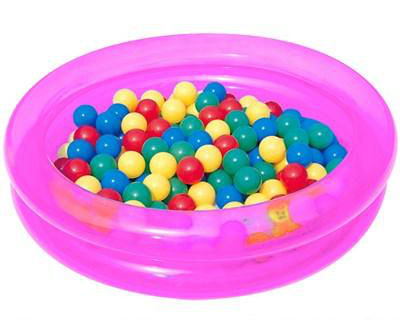
\includegraphics[height=3.5cm]{../figs/ballpool.png}
	\end{block}
\column{0.48\textwidth}
	\begin{block}{Statistics}
		\centering Given the colors of a few balls drawn, what can I know about the pool?\\
		\centering 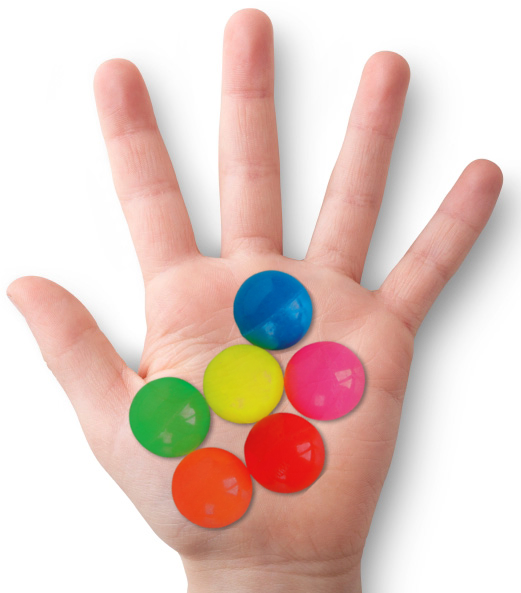
\includegraphics[height=3.45cm]{../figs/hand02.png}
	\end{block}
\end{columns}
\lfr{Pool image: \url{http://goo.gl/y8doaN}}
\end{ftst}

%=====

\begin{ftst}
{Population, Sample and Observation}
{Definitions}
\begin{columns}
\column[T]{0.85\textwidth}
``A \textbf{population} is a large set of objects of a similar nature which is of interest as a whole''$^{[1]}$. It can be an actual set (e.g., all balls in the pool) or a hypothetical one (e.g., all possible outcomes for an experiment).
\column[T]{0.15\textwidth}
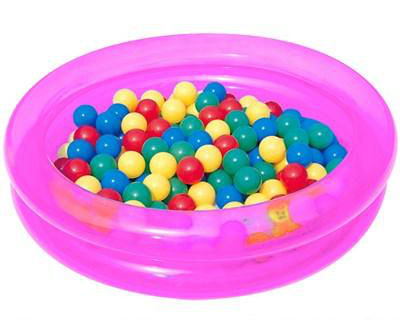
\includegraphics[width=\textwidth]{../figs/ballpool.png}
\end{columns}
\vone
\begin{columns}
\column[T]{0.12\textwidth}
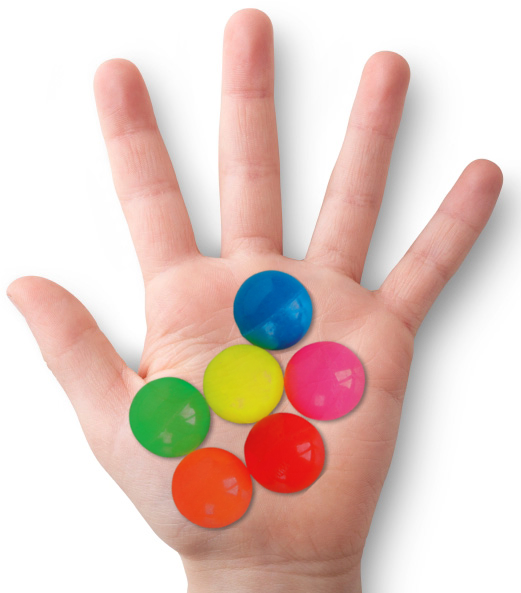
\includegraphics[width=\textwidth]{../figs/hand02.png}
\column[T]{0.88\textwidth}
\vhalf
A \textbf{sample} is a subset of a population. ``A sample is chosen to make inferences about the population by examining or measuring the elements in the sample''$^{[2]}$.
\end{columns}
\vone\vhalf
\begin{columns}
\column[T]{0.88\textwidth}
\vhalf
An \textbf{observation} is a single element of a given sample, an individually collected data point. An observation can also be considered as a sample of size one.
\column[T]{0.12\textwidth}
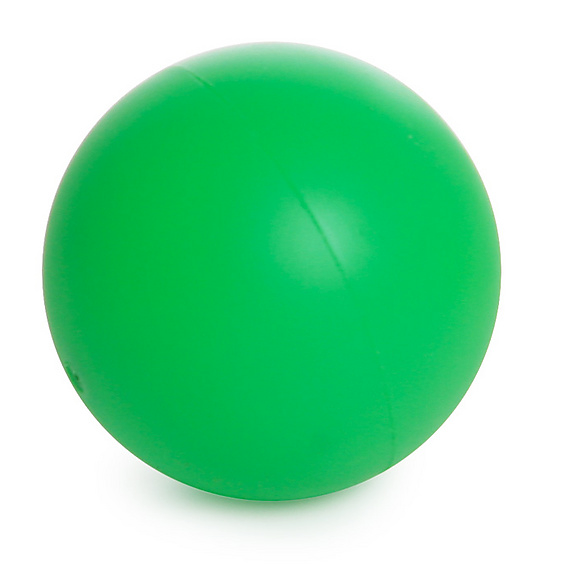
\includegraphics[width=\textwidth]{../figs/greenball.png}
\end{columns}
\lfr{Green ball: \url{http://goo.gl/Fb8Z68}}
\lfr{[1] Glossary of statistical terms: \url{http://www.statistics.com/glossary&term_id=812}}
\lfr{[2] Glossary of statistical terms: \url{http://www.statistics.com/glossary&term_id=274}}
\end{ftst}

%=====

\begin{ftst}
{Point and Interval Estimates}
{Basic concepts}
Two of the central concepts of statistical inference are \textit{point estimators} and \textit{statistical intervals}.
\vone
Both terms refer to using information obtained from a \textit{sample} to infer probable values about \textit{population} parameters;

\bitems \textbf{Point estimate}: estimated value for a given population parameter;
	\spitem \textbf{Statistical interval}: estimated interval of possible/probable values for a given population parameter; 
\eitem
\end{ftst}

%=====

\begin{ftst}
{Statistics and Sampling Distributions}
{Definition}
Suppose one wants to obtain a point estimate for an arbitrary parameter, e.g. the mean of a given population;
\vone
Randomly sampling from a population results in a random variable, and any function of these observations - that is, any \textit{statistic} - is consequently a random variable itself;
\vhalf
\begin{columns}
\column[T]{0.25\textwidth}
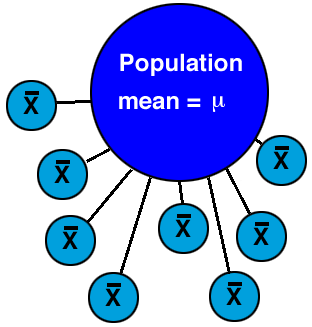
\includegraphics[width=\textwidth]{../figs/sam.png}
\column[T]{0.75\textwidth}
\vhalf
Being random variables means that statistics also have their own probability distributions, called \textit{sampling distributions}$^{[3]}$. Sampling distributions have specific characteristics that we'll explore later.
\end{columns}
\lfr{Image: \url{http://www.philender.com/courses/intro/notes2/sample.html}}
\lfr{[3] D.W. Stockburger: \url{http://www.psychstat.missouristate.edu/introbook/sbk19.htm}}
\end{ftst}

%=====

\begin{ftst}
{Point Estimators}
{Definition}
A \textit{point estimator} is a statistic which provides the value of maximum plausibility for a given (unknown) population parameter $\theta$.
\vone
Consider a random variable $X$ distributed according to a given $f(X|\theta)$.
\vone
Consider also a random sample from this variable: $\mbf{x}=\{x_1,x_2,\ldots,x_n\}$;
\vone
A given function $\hat{\Theta}=h\left(\mbf{x}\right)$ is called a \textit{point estimator} of the parameter $\theta$, and a value returned by this function for a given sample is referred to as a \textit{point estimate} $\hat{\theta}$ of the parameter.
\end{ftst}

%=====

\begin{ftst}
{Point Estimators}
{Usual cases}
Point estimation problems arise frequently in all areas of science and engineering, whenever there is a need for estimating, e.g.,:

\bitems a population  mean, $\mu$;
	\item a population variance, $\sigma^2$;
	\item a population proportion, $p$;
	\item the difference in the means of two populations, $\mu_1-\mu_2$; 
	\item etc..
\eitem
\vhalf
In each case there are multiple ways of performing the estimation task, and the decision about which estimators to use is based on the mathematical properties of each statistic.
\end{ftst}

%=====

\begin{ftst}
{Point Estimators}
{Unbiased estimators}
A good estimator should consistently generate estimates that lie close to the real value of the parameter $\theta$.
\vone
A given estimator $\hat{\Theta}$ is said to be \textit{unbiased} for parameter $\theta$ if:
\beqs
E\left[\hat{\Theta}\right] = \theta
\eqs
\noindent or, equivalently:
\beqs
E\left[\hat{\Theta}\right] - \theta = 0
\eqs
\vone
The difference $E\left[\hat{\Theta}\right] - \theta$ is referred to as the \textit{bias} of a given estimator.
\end{ftst}

%=====

\begin{ftst}
{Point Estimators}
{Unbiased estimators}
The usual estimators for mean and variance are unbiased estimators;
\vone
Let $x_1,\ldots,x_n$ be a random sample from a given population $X$, characterized by its mean $\mu$ and variance $\sigma^2$. In this situation, it is possible to show that$^{[4]}$:
\beqs
E\left[\bar{x}\right] = E\left[\frac{1}{n}\sum\limits_{i=1}^{n}x_i\right] = \mu
\eqs
\noindent and:
\beqs
E\left[s^2\right] = E\left[\frac{1}{n-1}\sum\limits_{i=1}^{n}\left(x_i-\bar{x}\right)^2\right] = \sigma^2
\eqs
\lfr{[4] For details see  S.D. Anderson (1999), \textit{Proof that Sample Variance is Unbiased}: \url{http://git.io/vUn9N}.}
\end{ftst}

%=====

\begin{ftst}
{Point Estimators}
{Unbiased estimators}
There usually exists more than one unbiased estimator for a given parameter $\theta$. The variances of these estimators may, however, be different
\vone
\begin{columns}[T]
    \column{0.5\textwidth}\vspace{-1.5em} 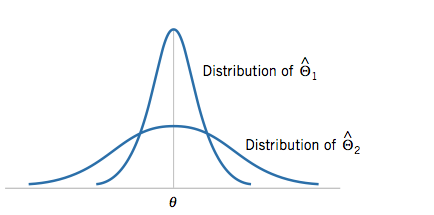
\includegraphics[width=1.2\textwidth]{../figs/ubes-var.png}
    \column{0.5\textwidth} A logical choice is to try to obtain the unbiased estimator of minimal variance. This is generally called the \textit{minimal-variance unbiased estimator} (MVUE).
\end{columns}
\vone
MVUE are generally chosen as estimators due to their ability of generating estimates $\hat{\theta}$ that are (relatively) close to the real value of $\theta$.
\lfr{Image: D.C.Montgomery,G.C. Runger, \textit{Applied Statistics and Probability for Engineers},Wiley 2003.}
\end{ftst}

%=====

\begin{ftst}
{Point Estimators}
{Standard error}
The \textit{standard error} of an estimator $\hat{\Theta}$ corresponds to the standard deviation of that estimator,
\beqs
\sigma_{\hat{\Theta}} = \sqrt{Var\left[\hat{\Theta}\right]}
\eqs
\vone
When the standard error is estimated from a given sample we refer to it as the \textit{estimated standard error},  $\hat{\sigma}_{\hat{\Theta}}$ (the notations $s_{\hat{\Theta}}$ and $se(\hat{\Theta})$ are also common).
\end{ftst}

%=====

\begin{ftst}
{Point Estimators}
{Standard error}
For the most usual point estimates used with Gaussian variables, we have:$^{[5]}$
\beqs
\hat{\sigma}_{\bar{X}} = \frac{s}{\sqrt{n}}
\eqs

\beqs
\hat{\sigma}_{S^2} = s^2\sqrt{\frac{2}{n-1}}
\eqs

\beqs
\hat{\sigma}_{S} = \frac{s}{\sqrt{2(n-1)}} + O\left(\frac{1}{n\sqrt{n}}\right)\approx \frac{s}{\sqrt{2(n-1)}}
\eqs

\vone
More general estimates of the standard error for different distributions (or different statistics) can usually be obtained using resampling strategies or asymptotic results.
\lfr{$[5]$ See Ahn and Fessler (2003), \textit{Standard Errors of Mean, Variance, and Standard Deviation Estimators}: \url{https://git.io/v5Z5v}}
\end{ftst}

%=====

\begin{ftst}
{Sampling Distributions}
{Sampling distributions of means}
Suppose a coaxial cable manufacturing operation that produces cables with a target resistance of $50\Omega$ and a standard deviation of $2\Omega$$^{[5]}$, and assume that the resistance values are distributed according to a known Normal distribution, i.e., $X\sim\mathcal{N}\left(\mu=50,\sigma^2=4\right)$. 
\vone
Also suppose a random sample of $25$ cables is taken from this production process and their resistance is measured. The sample mean of the observations taken,
\beqs
\bar{x} = \frac{1}{25}\sum\limits_{i=1}^{25}{x_i}
\eqs

\noindent is also normally distributed, with $E[\bar{x}] = \mu = 50\Omega$ (since the sample mean is an unbiased estimator) and $\sigma_{\bar{x}} = \sqrt{\sigma^2/25} = 0.4\Omega$.
\lfr{[5] Example inspired on \url{https://www.sas.com/resources/whitepaper/wp_4430.pdf}}
\end{ftst}

\begin{ftst}
{Sampling Distributions}
{The Central Limit Theorem}
Even for arbitrary population distributions the sampling distribution of means tends to be approximately normal (with $E[\bar{x}] = \mu $ and $s_{\bar{x}} = \sigma^2/n$). 
\vone
More generally, let $x_1,\ldots,x_n$ be a sequence of \textit{independent and identically distributed} (\textbf{iid}) random variables, with mean $\mu$ and finite variance $\sigma^2$. Then:
\beqs
z_n = \frac{\sum\limits_{i=1}^{n}{(x_i)} - n\mu}{\sqrt{n\sigma^2}} = \frac{\bar{x} - \mu}{\sqrt{\sigma^2/n}}
\eqs
\noindent is distributed asymptotically as a standard Normal variable, that is, $z_n\sim\mathcal{N}(0,1)$.
\lfr{For more details on the CLT, see \url{https://www.encyclopediaofmath.org/index.php/Central_limit_theorem}}
\end{ftst}

\begin{ftst}
{Sampling Distributions}
{The Central Limit Theorem}
This result is known as the \textit{Central Limit Theorem}, and is one of the most useful properties for statistical inference. The CLT allows the use of techniques based on the Normal distribution, even when the population under study is not normal.
\vone
For ``well-behaved'' distributions (continuous, symmetrical, unimodal - the usual bell-shaped pdf we all know and love) even small sample sizes are commonly enough to justify invoking the CLT and using parametric techniques.
\end{ftst}

\begin{ftst}
{Sampling Distributions}
{The Central Limit Theorem}
For an interactive demonstration of the CLT, download the files in {\small\url{https://git.io/vnPj8}} and run on RStudio.
\vone
{\centering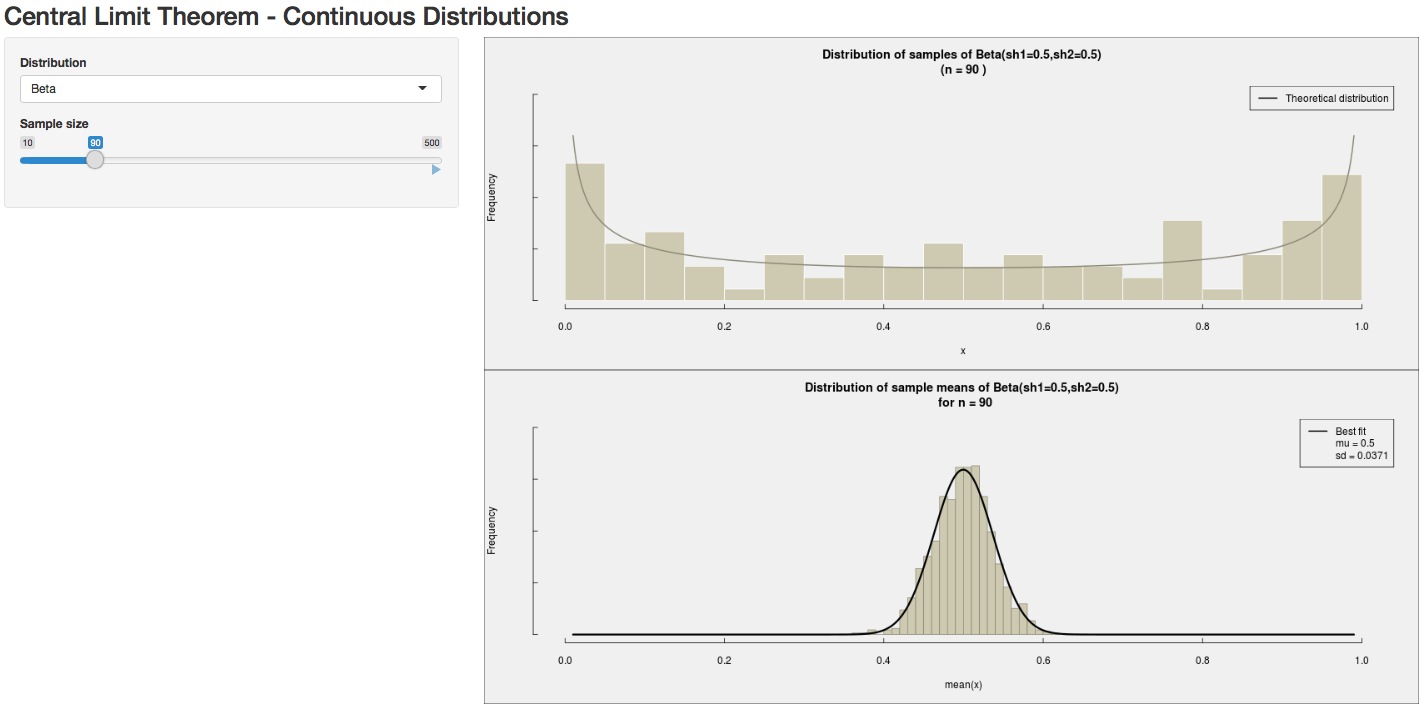
\includegraphics[width=\textwidth]{../figs/CLTdemo.png}}
\end{ftst}



\begin{ftst}
{Bibliography}
{\ }
\scriptsize
\textbf{Required reading}

\benums D.C. Montgomery and G.C. Runger, \textit{Applied Statistics and Probability for Engineers}, Chapter 7. 3rd Ed., Wiley 2005.
\item D.W. Stockburger, \textit{Sampling Distributions}. In: \textit{Introductory Statistics: Concepts, Models, and Applications} - \url{http://www.psychstat.missouristate.edu/introbook/sbk19.htm}
\eenum

\textbf{Recommended reading}

\benums R. Willett, \textit{ ECE 830 Estimation and Decision Theory, Spring 2014}, Chapters 13-15 - \url{http://willett.ece.wisc.edu/education.html}
\item S. Okasha, \textit{Philosophy of Science - a very brief introduction}, Oxford Paperbacks, 2002.
\eenum
\end{ftst}

%=====

\begin{ftstf}{About this material}{Conditions of use and referencing}
\centering\footnotesize This work is licensed under the Creative Commons CC BY-NC-SA 4.0 license\\(Attribution Non-Commercial Share Alike International License version 4.0).\\
\vhalf
\url{http://creativecommons.org/licenses/by-nc-sa/4.0/}\\
\vone
\footnotesize Please reference this work as:\\
\footnotesize \flushleft Felipe Campelo (2018), \textit{Lecture Notes on Design and Analysis of Experiments}.\\Online: {\scriptsize\url{https://github.com/fcampelo/Design-and-Analysis-of-Experiments}}\\
Version 2.12. Creative Commons BY-NC-SA 4.0.\\

\begin{Verbatim}[fontsize=\tiny]
    @Misc{Campelo2018,
      title={Lecture Notes on Design and Analysis of Experiments},
      author={Felipe Campelo},
      howPublished={\url{https://github.com/fcampelo/Design-and-Analysis-of-Experiments}},
      year={2018},
      note={Version 2.12. Creative Commons BY-NC-SA 4.0.},
    }
\end{Verbatim}

\begin{tikzpicture} [remember picture,overlay]
\node[anchor=south,yshift=0pt] at (current page.south){ \includegraphics[width=.2\textwidth]{../figs/CCSomerights.png}};
\end{tikzpicture}
\end{ftstf}


\end{document}